\chapter{Introduction} \label{chap:intro}
Fracture toughness is a material property that quantifies the material's resistance to crack growth.
Fracture toughness in cracked bodies can be divided into three main categories of behavior: linear elastic, elastic-plastic, or fully-plastic, as seen in \Cref{fig:lefm-epfm-fp}.
Linear elastic fracture applies when the size of the yield zone and deformations near the crack tip are small compared to the dimensions of the body, allowing certain simplifying assumptions to apply.
Elastic-plastic fracture applies when the size of the yield zone and deformations near the crack tip are large enough to invalidate the simplifying assumptions of linear elastic fracture theory.
Fully-plastic fracture applies when the size of the yield zone extends far beyond the crack tip and stress and strain fields near the crack tip are indistinguishable from those further away.
Linear elastic materials are typically brittle, and fully-plastic materials severely deform once they reach their yield strength.
Of these categories, elastic-plastic fracture is particularly relevant to both aerospace components (particularly engines)
which operate at both high temperatures and high stresses, and in the nuclear power industry where elastic-plastic fracture mechanics was first applied.
As with many nonlinear mechanics problems, elastic-plastic fracture mechanics presents a great set of challenges for design, testing, and simulation.
\begin{figure}[tbp]
\centering
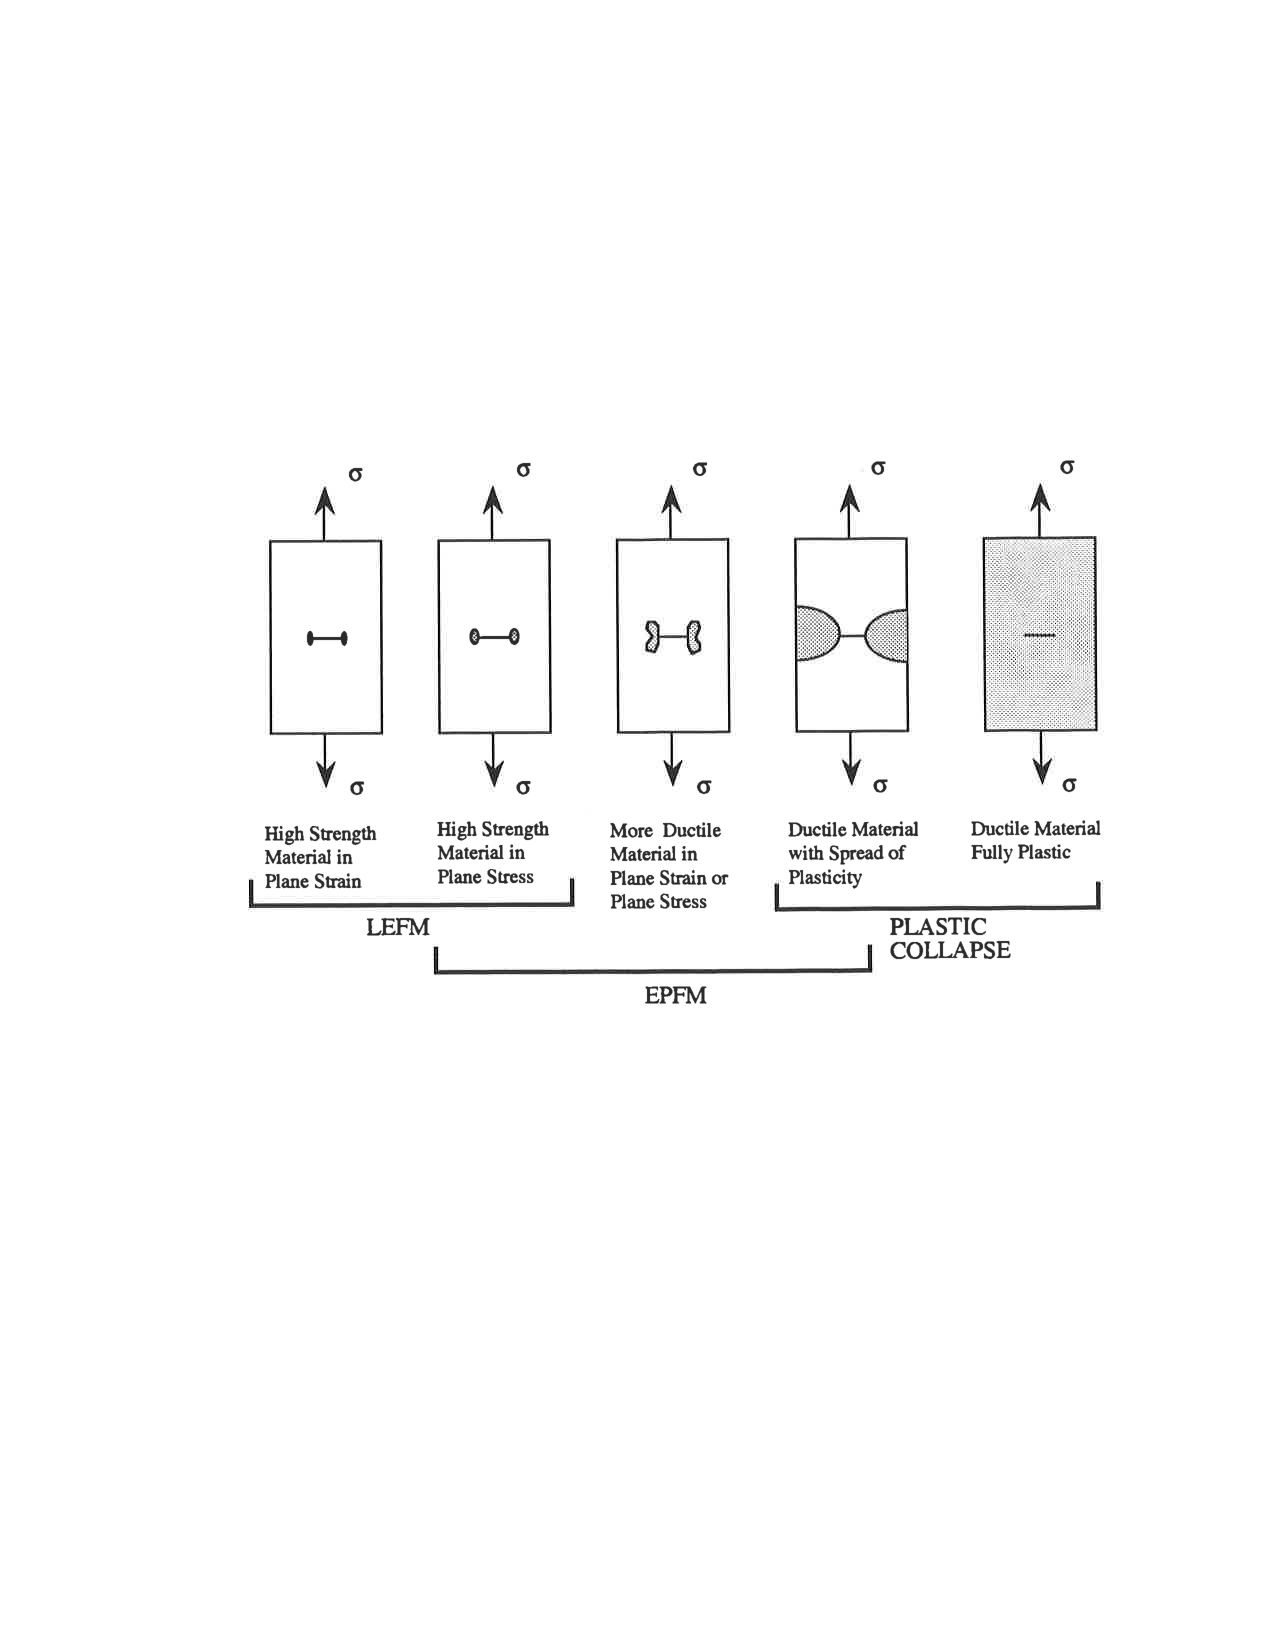
\includegraphics[width=0.7\columnwidth]{lefm-epfm-fp}
\caption[Categories of Fracture Mechanics Behaviors]{\label{fig:lefm-epfm-fp} Categories of Fracture Mechanics Behaviors \cite{janssenzuidemawanhill2002}}
\end{figure}

One of the significant challenges is to experimentally determine fracture toughness under elastic-plastic conditions.
This challenge is compounded by curved crack fronts, such as a surface crack in a plate subjected to tension or bending.
While test standards such as ASTM E399 ``Standard Test Method for Linear-Elastic Plane-Strain Fracture Toughness \KIc of Metallic Materials''~\cite{astme399} and ASTM E1820 ``Standard Test Method for Measurement of Fracture Toughness''~\cite{astme1820} are used for test specimen geometries with through cracks (a crack that goes completely through the cross section), test specimen geometries with surface cracks require an additional level of complexity.
ASTM E740 ``Standard Practice for Fracture Testing with Surface-Crack Tension Specimens''~\cite{astme740} addresses surface cracks, but only for linear elastic materials.
ASTM E399, ASTM E740, and ASTM E1820 have all reached a level of maturity and use but none address surface crack geometries for elastic-plastic materials.
ASTM E2899\footnote{As of November 2018, the current revision of ASTM E2899 was \href{https://www.astm.org/Standards/E2899.htm}{E2899-15}.} ``Standard Test Method for Measurement of Initiation Toughness in Surface Cracks Under Tension and Bending''~\cite{astme2899} was developed specifically to address surface crack geometries in tension and bending for elastic-plastic materials.
A supporting analysis tool for tension has been developed by Allen of NASA~\cite{allenwells2014}.
However, the tool does not include the supporting analysis to easily perform measurement of fracture toughness in bending.

The motivation of this research is to address the shortcomings of ASTM E2899 with regard to fracture toughness of surface cracks in flat plates subjected to bending.
In doing so, the current research must closely follow established techniques in verification and validation to ensure accurate results suitable for a range of crack shape geometries and elastic-plastic materials.
The primary goal of this research is to extend the existing tool to support bending conditions.

\section{Surface Cracks}

Surface cracks such as the one shown in \Cref{fig:sc-terminology-e2899} are some of the most common discontinuities found in structural components, and can be caused by scratches, surface finish quality, tool strikes, welding procedures, and other phenomena.
\begin{figure}[tbp]
\centering
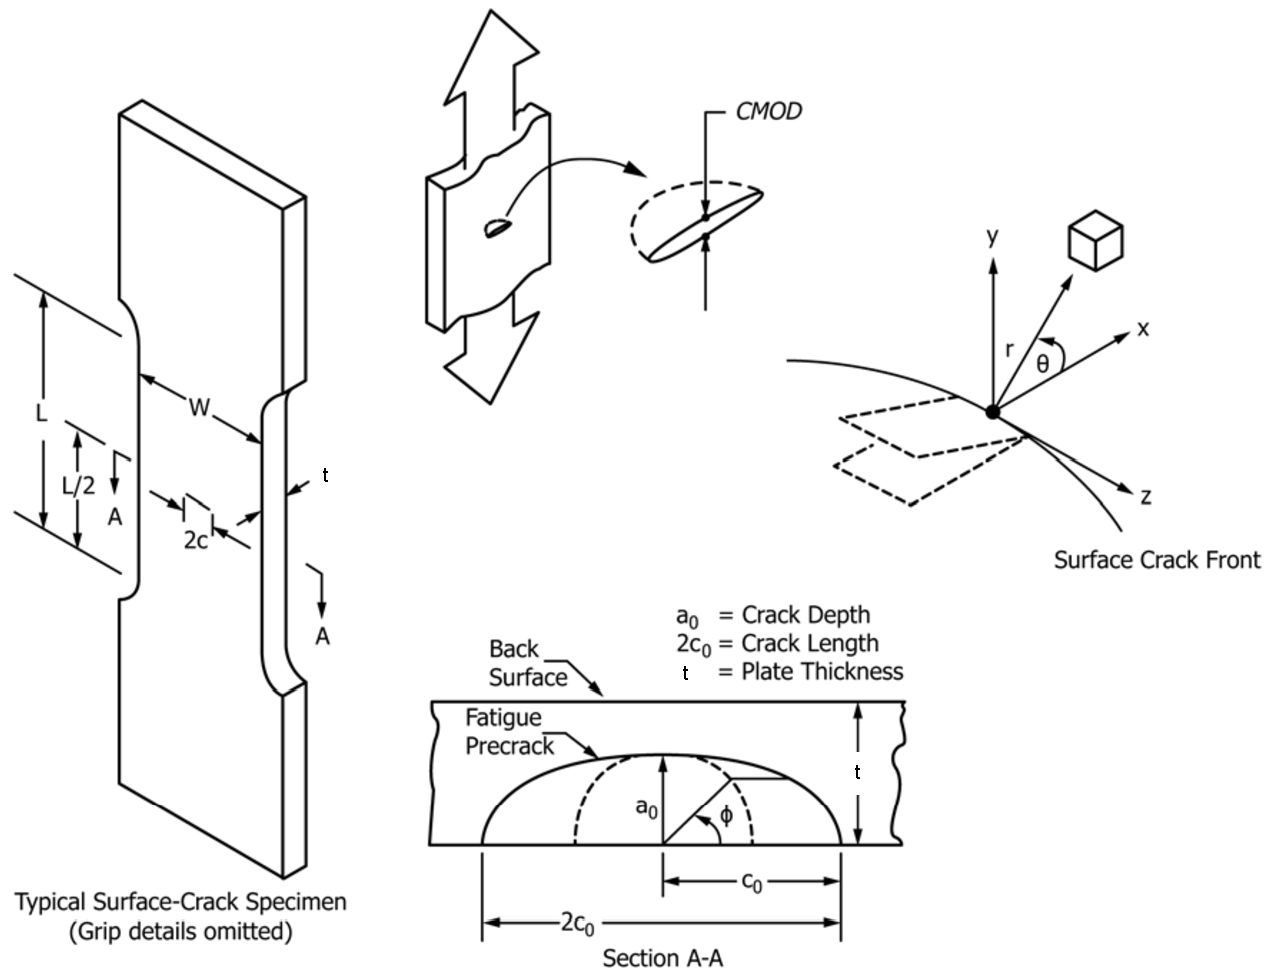
\includegraphics[width=0.95\columnwidth]{sc-terminology-e2899-modified}
\caption[ASTM E2899 Test Specimen and Crack Configurations]{\label{fig:sc-terminology-e2899} ASTM E2899 Test Specimen and Crack Configurations \cite{astme2899}}
\end{figure}
Surface crack geometry is inherently three-dimensional and the stress states around the perimeter of the crack can vary from a practically plane-stress state on the free surface to a practically plane-strain state at the deepest part of the crack.
Computationally, the modeling of stress state and fracture criteria around the perimeter of a surface crack requires a fine level of discretization not required for two-dimensional edge cracks or center cracks.

Surface cracks (especially surface cracks in bending) are subject to a wide range of local stress conditions beyond the plane-stress/plane-strain distinction.
These localized conditions are defined as constraint, and affect the influence of the Poisson effect on deformation and strain.
Where constraint levels are high, a hydrostatic stress state exists that allows higher stresses to develop without a corresponding amount of localized yielding or plastic deformation.
The constraint may lead to lower measurements of fracture toughness compared to an otherwise identical region of material subject to less constraint.
In regions with high constraint, the linear elastic stress intensity \K or the elastic-plastic strain energy release rate \J accurately predicts crack growth or failure, and the exact level of constraint has little effect on toughness measurements.
In regions with low constraint, \K or \J is coupled with a constraint measure (\(Q\), \(\Omega\), or a normalized Williams \(T\) stress) to predict crack growth or failure, as seen in \Cref{fig:toughness-constraint-locus}.
\begin{figure}[tbp]
\centering
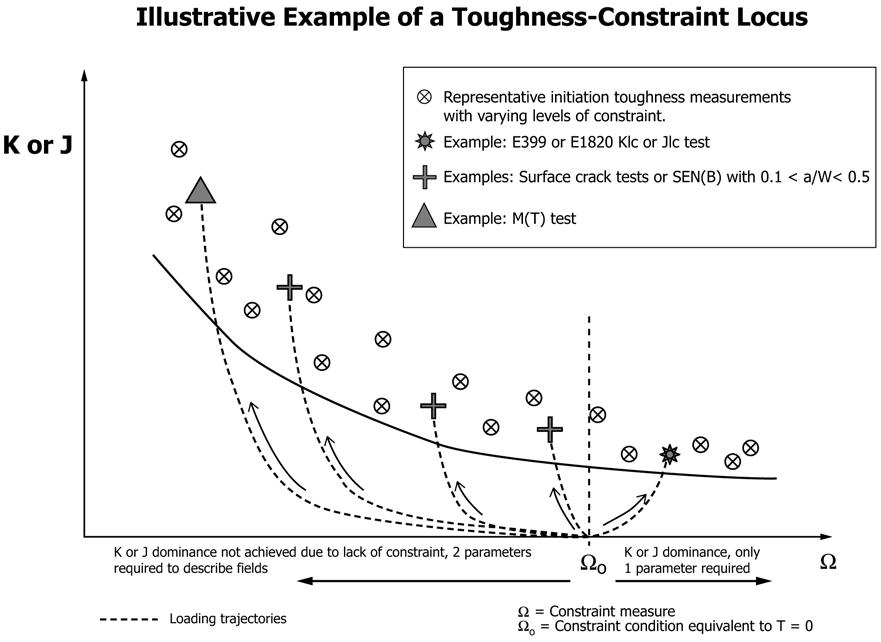
\includegraphics[width=0.9\columnwidth]{toughness-constraint-locus}
\caption[Example of Toughness-Constraint Locus]{\label{fig:toughness-constraint-locus} Example of Toughness-Constraint Locus \cite{astme2899}}
\end{figure}

The semi-elliptical surface crack in a flat plate is one of the simpler types of part-through cracks, and \Cref{fig:nasgro-geometries} show other types of surface cracks, including those at corners, in spheres, or in solid or hollow cylinders.
Handbook or other curve-fitted solutions exist for all these geometries, but only for linear elastic materials.
Regardless of the specific geometry, all these geometries exhibit varying levels of constraint around the crack front, and no simple solutions exist for characterizing their elastic-plastic fracture properties.
\begin{figure}[tbp]
\centering
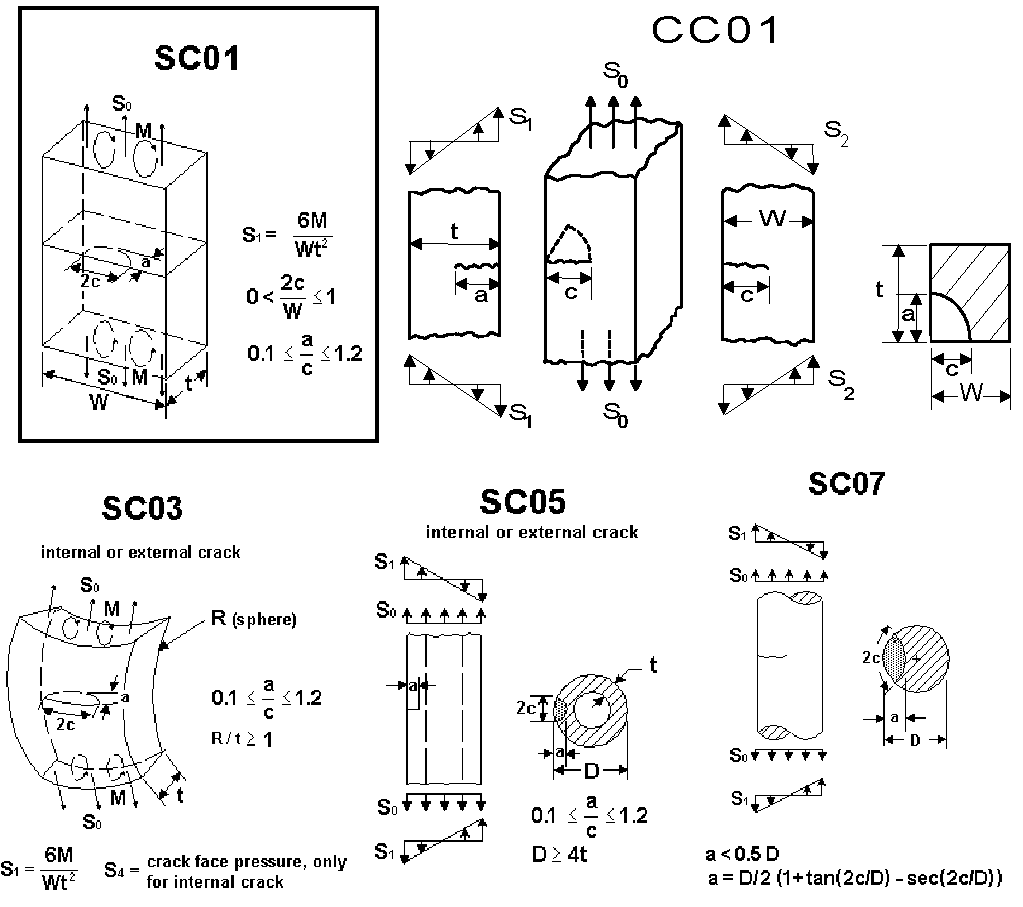
\includegraphics[width=0.8\columnwidth]{nasgro-geometries}
\caption[NASGRO Surface Crack Geometries]{\label{fig:nasgro-geometries} NASGRO Surface Crack Geometries \cite{nasgro2000}}
\end{figure}

\section{Mechanical Properties and Fracture Toughness Standards}

Several standards for evaluating mechanical properties, including fracture toughness, have been developed by ASTM International and other standards bodies.
These standards are predominantly experimental, with limited calculations and analysis required.
Both ASTM E8, ``Standard Test Methods for Tension Testing of Metallic Materials,''~\cite{astme8} ASTM E399, ``Standard Test Method for Linear-Elastic Plane-Strain Fracture Toughness \KIc of Metallic Materials,''~\cite{astme399}, and ASTM E740, ``Standard Practice for Fracture Testing with Surface-Crack Tension Specimens,''~\cite{astme740} all use linear curve fits and basic calculations that could be completed with a strip chart and a calculator.
ASTM E1820, ``Standard Test Method for Measurement of Fracture Toughness,''~\cite{astme1820} uses a series of equations to calculate \K and an elastic component of \J, and calculates a plastic component of \J from the area under a load-displacement curve. These calculations could be completed with a spreadsheet.
ASTM E2899 details methods for measuring fracture toughness in flat specimens like those shown in \Cref{fig:sc-terminology-e2899}.
ASTM E2899 is a major departure from earlier standards in that it requires an elastic-plastic finite element analysis to calculate required \J values.
In 2014, one year after the initial release of ASTM E2899, Phillip Allen of NASA Marshall Space Flight Center released the Tool for the Analysis of Surface Cracks program (TASC) to help meet the analysis requirements of the standard.
TASC uses a database of finite element results for 600 surface-cracked plates covering a wide range of crack geometries and plate material properties, and interpolates results for intermediate geometries and material properties from the database.
This reduces the difficulty of complying with ASTM E2899, but the 2014 TASC program only applies to flat plates in tension, not in bending.

\section{Research Goals}
\label{sec:research-goals}

As of 2018, fracture toughness of a body with a surface crack can be readily evaluated for linear elastic materials in tension or bending by using handbook equations, or for elastic-plastic materials in tension by using TASC.
No such method exists for elastic-plastic materials in bending, so the primary goal of this research will be to create a database equivalent to the TASC tension database, and to modify the existing TASC program to support bending experiments.
To help ensure high quality results, a literature review in \Cref{chap:literature-review} includes consensus solutions for calculation of stress intensity factors, numerical methods for elastic-plastic and fully-plastic fracture mechanics of plates in bending, and techniques for verification and validation of results.
A short verification of tensile surface crack problems in \Cref{sec:verification-tasc} demonstrates techniques used to develop the bending model database.
The development of the bending database is detailed in \Cref{chap:research-plan}, including defining the plate models in terms of a few fundamental parameters, modifying boundary conditions to reach sufficient levels of elastic-plastic behavior, and extracting and compiling necessary results from the simulations into a the final database and modified version of TASC.
A set of force versus crack mouth opening displacement (CMOD)\nomenclature[1CMOD]{CMOD}{crack mouth opening displacement} data from a NASA tensile test is shown in \Cref{fig:force-cmod-phase-1}, and was used to judge finite element results from a variety of laboratories as part of a round-robin survey of surface crack modeling techniques shown in \Cref{fig:force-cmod-models-phase-1} \citep{wells2012analytical}.
Comparable data from a NASA bend test \cite{allen2018} is given in \Cref{fig:nasa-bend-p-cmod}, and it was used as a validation case in \Cref{chap:results}.
\begin{sidewaysfigure}
\centering
\begin{minipage}[b]{0.45\textwidth}
\centering
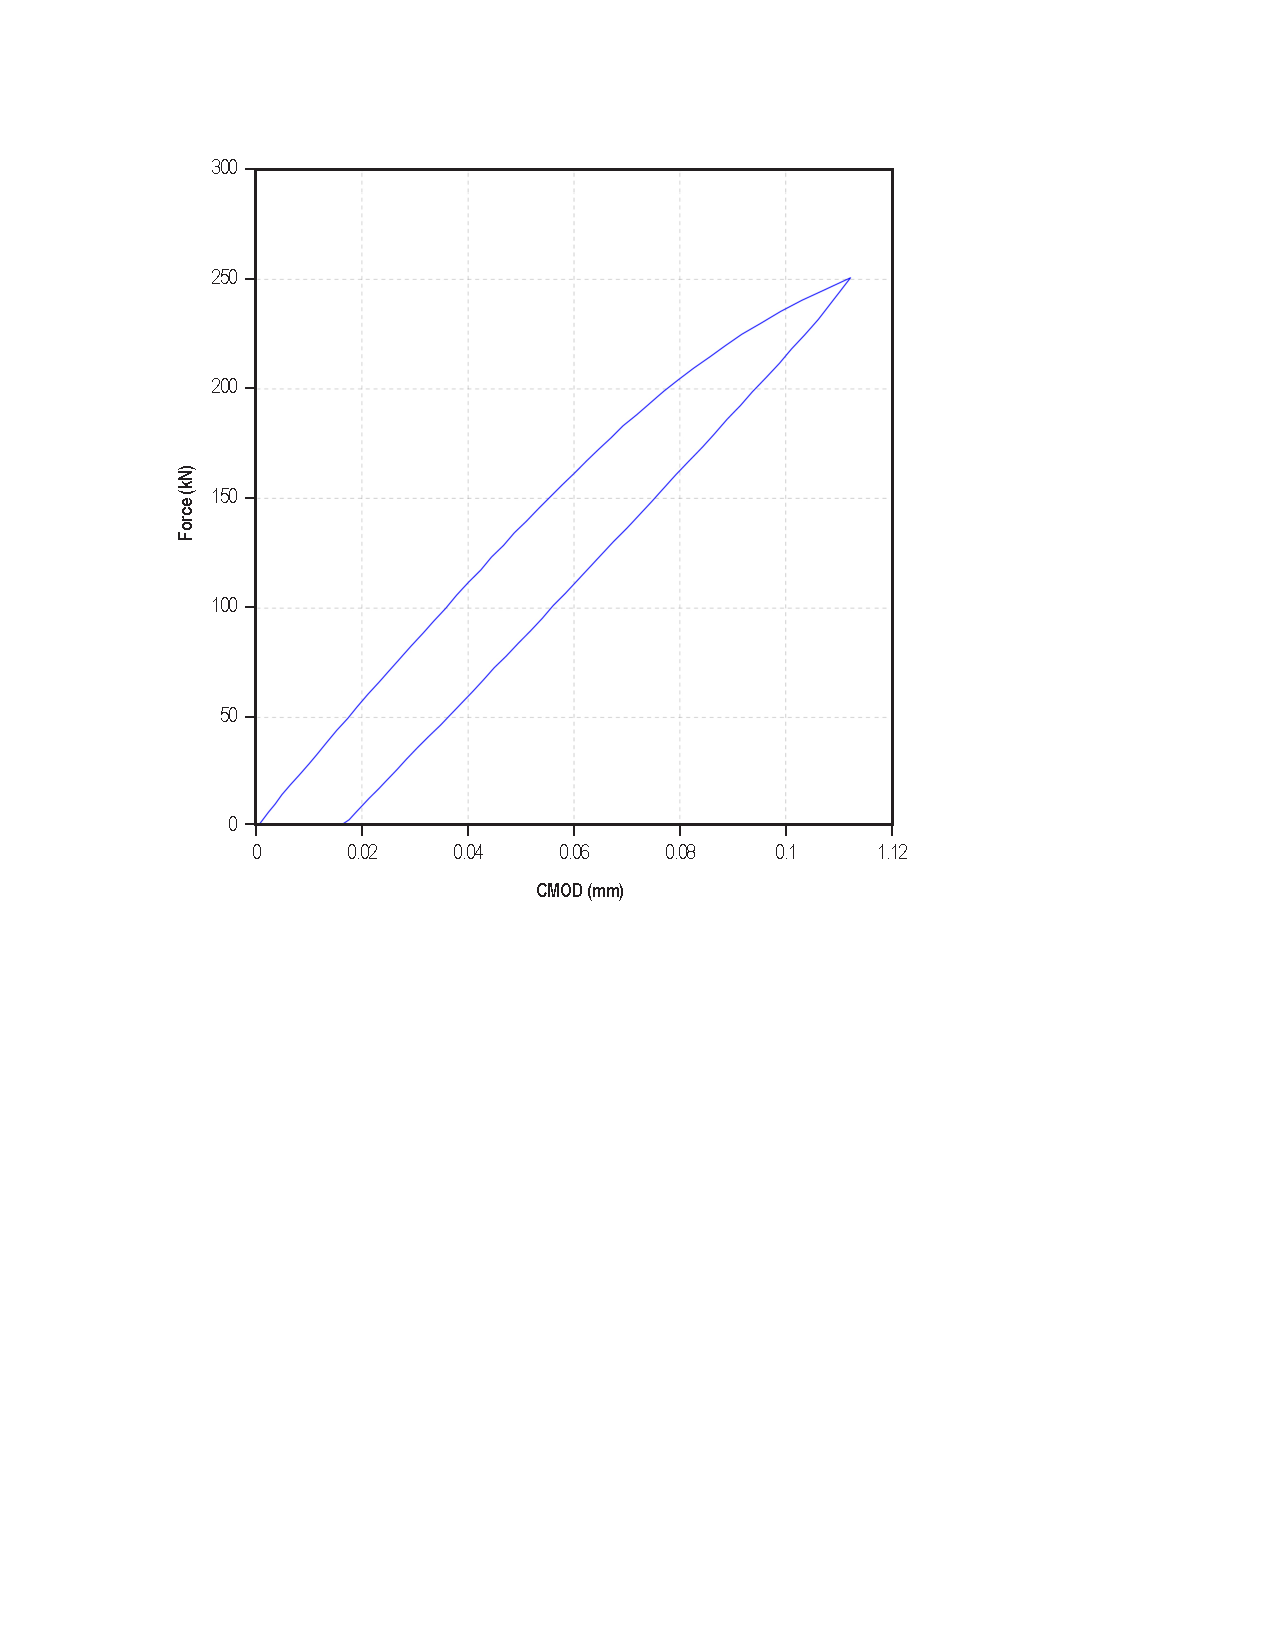
\includegraphics[height=3.64in]{force-cmod-phase-1}
\subcaption{\label{fig:force-cmod-phase-1} Tensile test}
\end{minipage}%
\begin{minipage}[b]{0.55\textwidth}
\centering
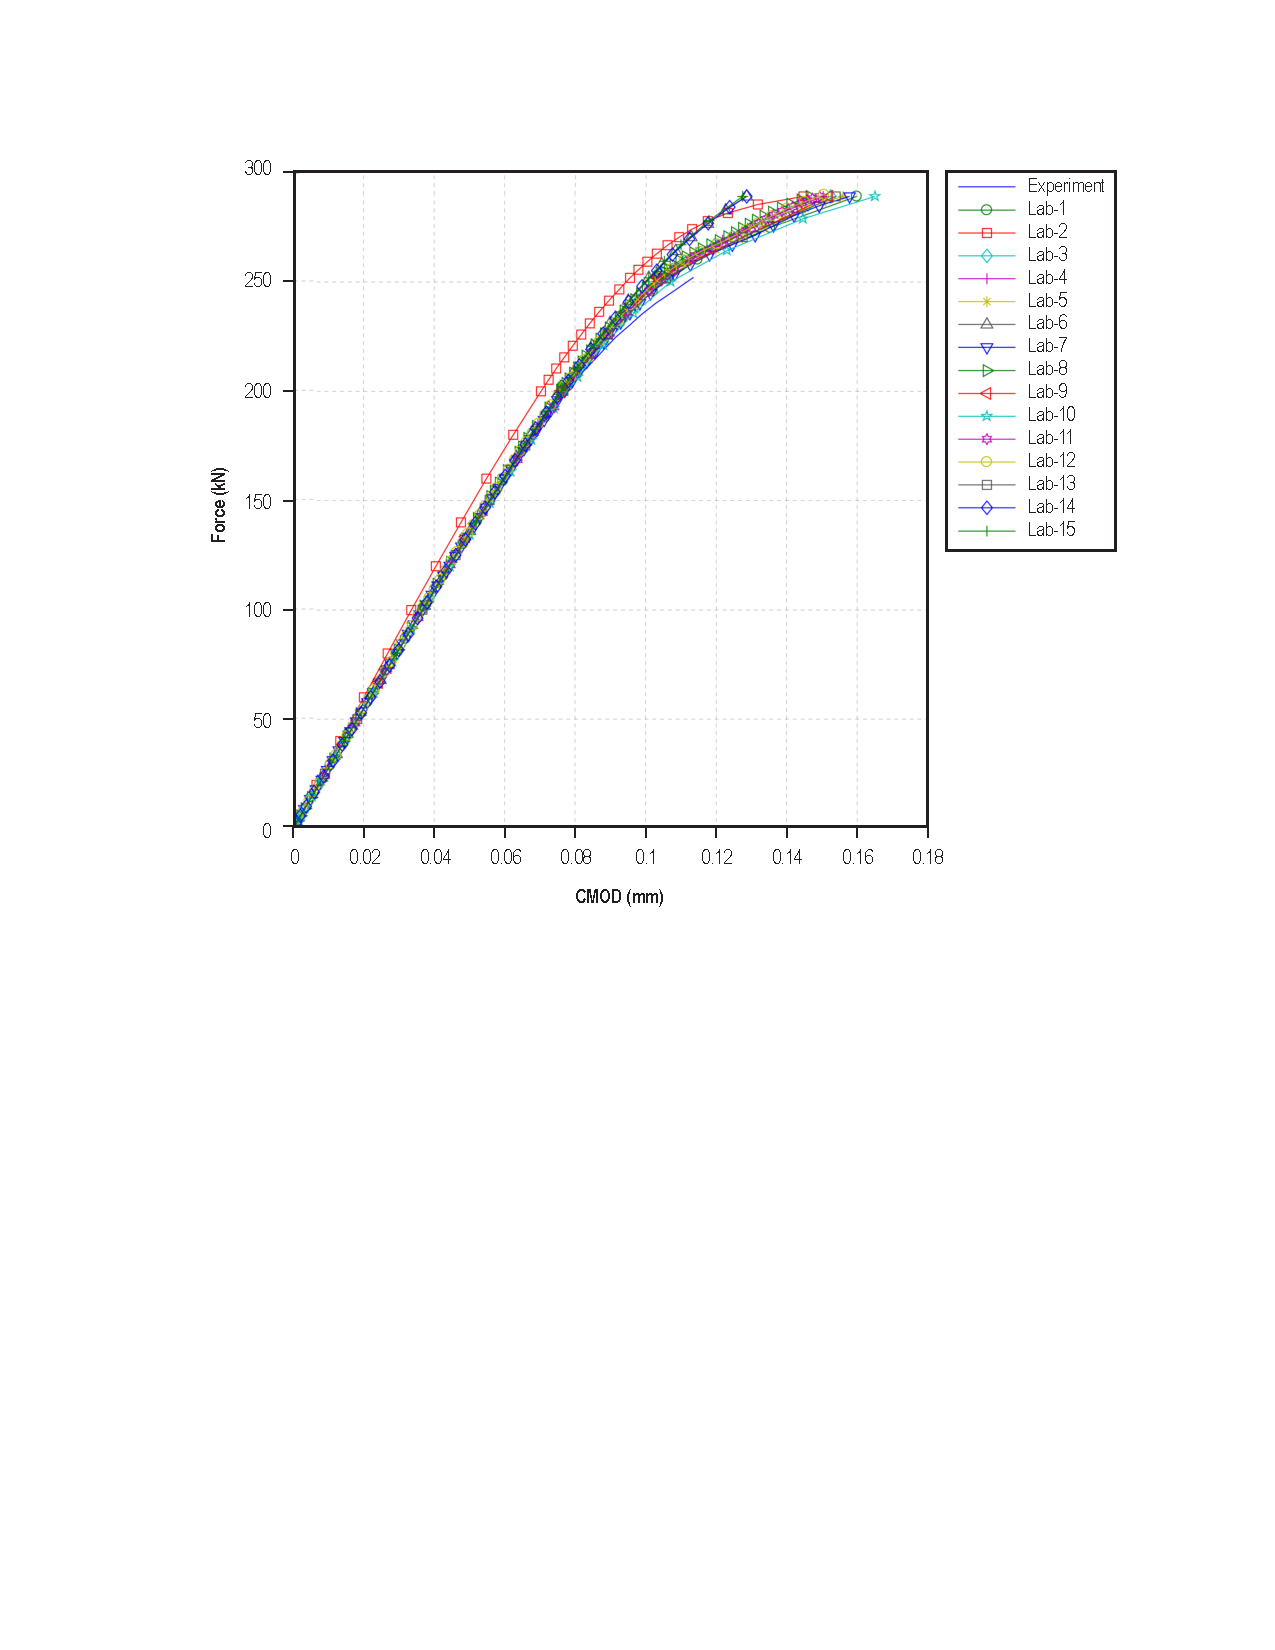
\includegraphics[height=3.64in]{force-cmod-models-phase-1}
\subcaption{\label{fig:force-cmod-models-phase-1} Comparison of finite element results to tensile test}
\end{minipage}
\caption[Force versus CMOD data from NASA experiment and round-robin finite element results]{Force versus CMOD data from NASA experiment and round-robin finite element results \citep{wells2012analytical}}
\end{sidewaysfigure}
\begin{figure}
\centering
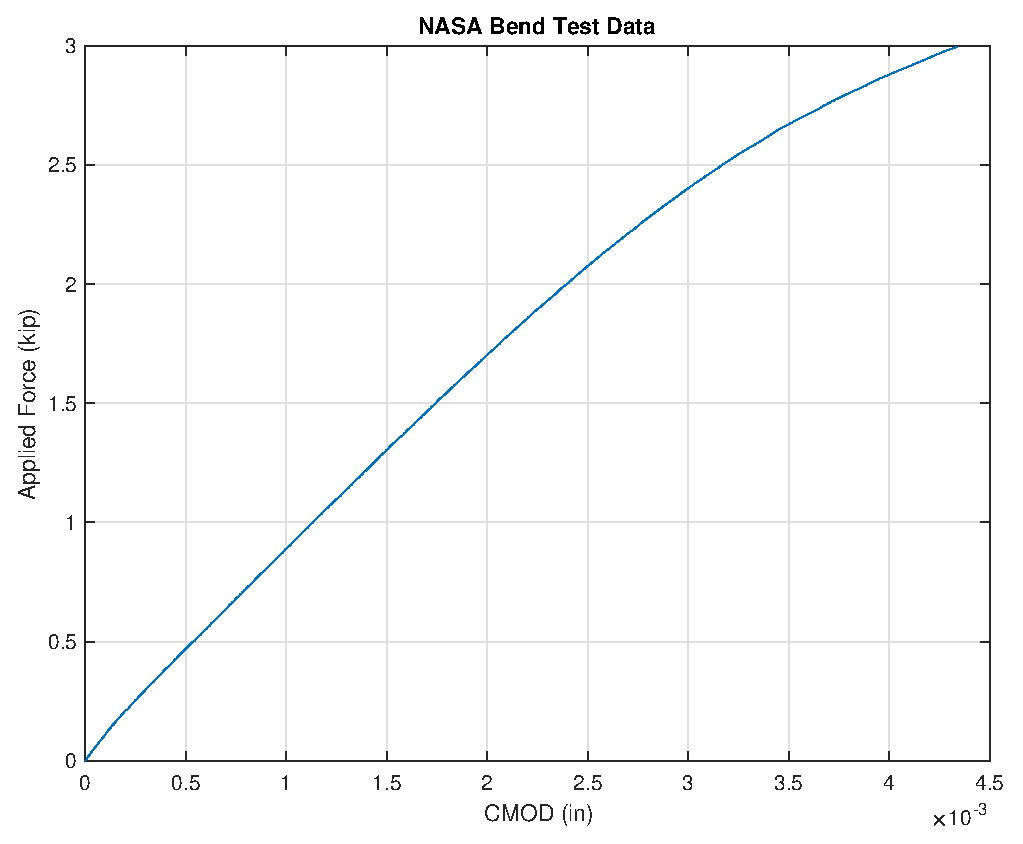
\includegraphics[width=\columnwidth]{nasa_bend_p_cmod}
\caption{\label{fig:nasa-bend-p-cmod} Force versus CMOD data from NASA bend test}
\end{figure}

The second goal of this research is an investigation of the applicability of estimating the elastic-plastic \J by summing elastic and fully-plastic \J values originally developed by the Electric Power Research Institute (EPRI)\nomenclature[1E]{EPRI}{Electric Power Research Institute}.
\Cref{sec:estimation} gives an overview of the EPRI estimation scheme,
\Cref{sec:h1-verification} summarizes some early work done with the EPRI technique for surface cracks in tension,
\Cref{chap:h1} briefly outlines plans for further verifications of the EPRI method,
and
\Cref{sec:epri-results} shows the results of the study.

The final goal of this research is an investigation of the applicability of the load separation technique~\citep{sharobeamlandes1991} to surface cracks in bending.
The load separation technique is a method analogous to separation of variables where the geometry-specific factors affecting \J are separated from the material-specific parameters affecting \J.
As seen in \Cref{fig:loadsep}, it results in a single-specimen technique that predicts behavior of a range of crack geometries for a given material.
Load separation was originally an experimental technique, but may also be applied to numerical models.
\begin{figure}[tbp]
\centering%
\begin{minipage}[t]{0.45\columnwidth}%
\centering%
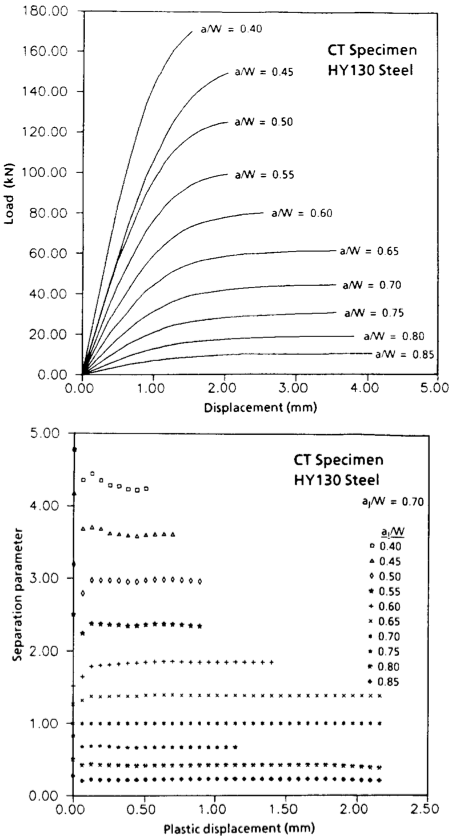
\includegraphics[width=\columnwidth]{load-sep-final}
\subcaption{Separation parameters}%
\end{minipage}%
\begin{minipage}[t]{0.45\columnwidth}%
\centering%
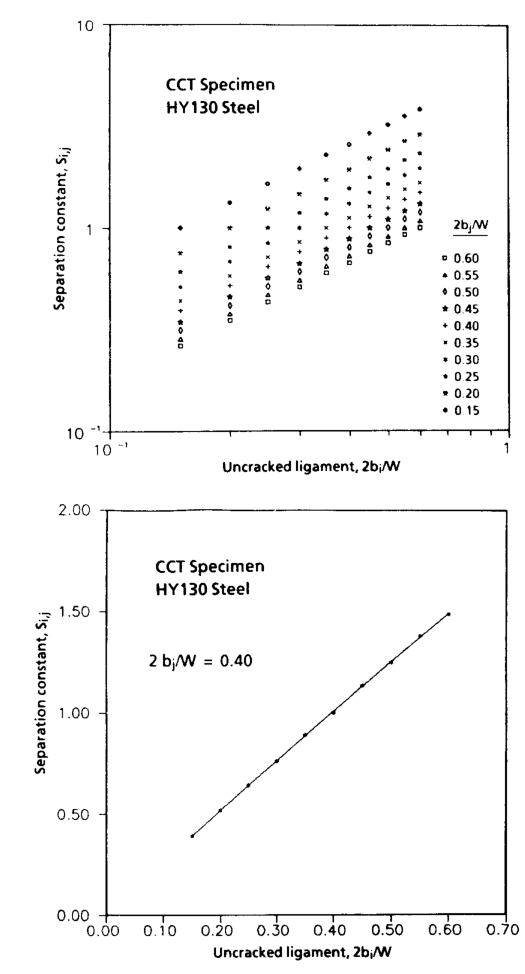
\includegraphics[width=\columnwidth]{load-separation-uncracked-ligament}%
\subcaption{Key curve for single-specimen technique}%
\end{minipage}%
\caption[Load separation technique]{\label{fig:loadsep} Load separation technique \citep{sharobeamlandes1991}}%
\end{figure}
An introduction to load separation is given in \Cref{sec:intro-load-separation}, 
the results of \citeauthor{sharobeamlandes1993}' study of surface cracks in tension \cite{sharobeamlandes1993} are replicated in \Cref{sec:loadsepverification},
\Cref{chap:load-separation} presents the plan for a more extensive study of load separation for surface cracks in bending,
and
\Cref{sec:results-loadsep} shows the results of the bending study.
